\documentclass[]{article}

\usepackage{graphicx}
\usepackage{caption}
\usepackage{subfig}
\usepackage{listings}

%opening
\title{Systems Biology Project 3}
\author{Mathias D. Kallick}

\begin{document}

\maketitle

\section{Genetic Algorithms}
Genetic algorithms are a computational technique used in Systems Biology to fit parameters to a model. Instead of relying on manually selected parameters, or something like a grid-search, where sets of parameters evenly covering the parameter space are tested, genetic algorithms rely on a more biologically inspired algorithm to speed up parameter fitting. In a genetic algorithm, you start by generating a set of parents, which are simply parameter sets that we can run the model with. We test each parameter set against a cost function, and in doing so determine how "good" that parameter set is. In a genetic algorithm, the quality of the parent determines the likelihood that it will be used as a parent for the next generation, but even the worst parent can be selected to generate a child. For the next generation, you pick parents according to a selection method, then you use those to generate the children (in our case, this means randomly mixing the parameters), and then you perturb each parameter a little bit to vary the data. You then do this for multiple generations, and because you make better parents more likely to be chosen to create children, each generation gets progressively better. In this way, a genetic algorithm can generate a very good parameter set without requiring exhaustive searching of a parameter space for the best parameters. It is also much less likely than a greedy algorithm to hit a local "best" parameter set that doesn't actually provide relatively good performance compared to the theoretical optimum parameters.

\subsection{Cost Function}
To use genetic algorithms (or an evolutionary strategy), there must be a way to quantify the "goodness" of a parameter set. This is the job of a cost function, which takes the parameters and returns a cost (low for a good fit, high for a bad one). In our case, this involves running the model with that parameter set for $800$ hours with a dt of $.1$ (this is where a lot of the time cost complexity comes in). I then calculate the period and amplitude of the second half of that data (allowing the first half as a startup period where the oscillations stabilize), and check them against the desired period and amplitude. I want a period of $23.6$ hours, and an amplitude that is not lower than $.1$.

\subsection{Elite Carryover}

\subsection{Selection Methods}
Selection methods are an important part of any genetic algorithm. Essentially, they represent the way that parents are selected for each child in the next generation. In my code, we first pick all of the parents for the next generation (some parents can be used multiple times, and it is also possible that a child has two of the same parent), and then generate the children with those parents.
\subsubsection{Tournament Selection}
Tournament selection is a way of picking lots of "local best" parents, which decreases the likelihood of a single "best" parameter set being beelined towards. Instead it provides some diversity in the resulting parameter sets. The idea behind tournament selection is to pick groups of children from the previous generation and find the best performer among each group (which is a small subset of the total child population). The best performers are then used as the parents of the next generation. The other advantage to tournament selection is that you never have to sort the list entirely. Thus, you get a better time complexity, because you only have to sort small subsets of the list, and sorting a list has a high time complexity. \\

In my test, tournament selection was capable of reducing cost by approximately $-2.19E-05$ per generation (starting at a cost of $1.54E-04$, and ending at $1.28E-06$, over $8$ generations). I noticed that tournament selection tended to find a good cost pretty quickly, but then got stuck on it for a while, staying constant for a few generations before finding a better one. \\

I also found that each generation took about 15 seconds to run, on my machine. \\

See Figure \ref{fig:ts1.1} for the plot generated using the parameters found with tournament selection.

\begin{figure}[!htbp]
	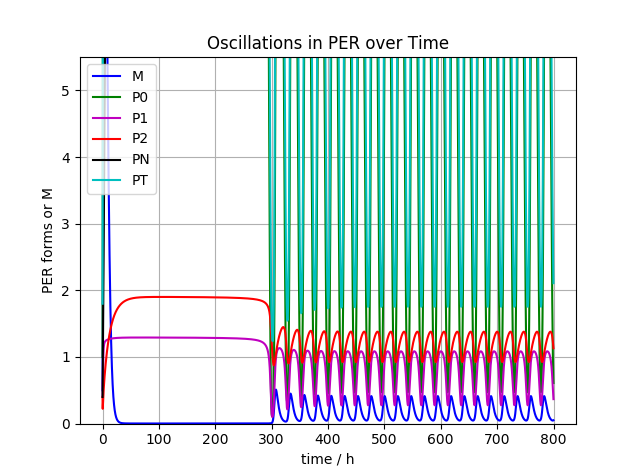
\includegraphics[width=\linewidth]{{"../plots/tourney_1.1"}.png}
	\caption{A simulation of the Goldbeter fly model using parameters (found with tournament selection): $n$ : $8.91$, $K_1$ : $8.67$, $K_2$ : $6.53$, $K_3$ : $1.00$, $K_4$ : $6.21$, $K_m$ : $7.09$, $K_d$ : $9.15$, $K_I$ : $5.48$, $V_1$ : $9.35$, $V_2$ : $6.43$, $V_3$ : $6.94$, $V_4$ : $1.72$, $v_m$ : $5.52$, $v_d$ : $6.22$, $v_s$ : $2.06$, $k_1$ : $8.55$, $k_2$ : $7.74$, $k_s$ : $3.36$}
	\label{fig:ts1.1}
\end{figure}
\subsubsection{Linear Ranking Selection}
Linear Ranking Selection is designed to allow any parents to be selected for the next generation, while making it more likely for the best ones to be chosen. The general idea is to sort the parents by quality, and then use a linear function to give each one a probability of being chosen - that makes the best one most likely to be chosen, but doesn't make it so unlikely to pick the worst parents that they never get chosen. This provides good diversity while also allowing for consistent improvement across generations. This selection method has one distinct disadvantage over tournament selection, which is that it requires a full sort of the parents, which increases the amount of time it needs to run. \\

In my test, linear ranking selection was capable of reducing cost by approximately $-4.73E-05$ per generation (starting at a cost of $3.82E-04$, and ending at $5.11E-05$, over $8$ generations). I noticed that linear selection was far more likely to get stuck on a particular parameter set - it would often stay on the same one for all $8$ generations, and most commonly only go through $2$ or $3$ sets in all of the generations. \\

I also found that each generation took about 16 seconds to run, on my machine. \\

See Figure \ref{fig:lr1.1} for the plot generated using the parameters found with linear ranking selection.

\begin{figure}[!htbp]
	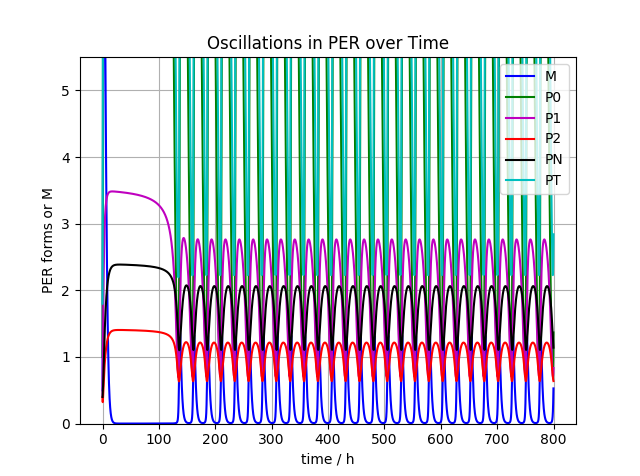
\includegraphics[width=\linewidth]{{"../plots/linear_1.1"}.png}
	\caption{A simulation of the Goldbeter fly model using parameters (found with linear ranking selection): $n$ : $7.79$, $K_1$ : $4.72$, $K_2$ : $4.42$, $K_3$ : $3.23$, $K_4$ : $7.68$, $K_m$ : $9.71$, $K_d$ : $3.14$, $K_I$ : $5.93$, $V_1$ : $9.24$, $V_2$ : $3.68$, $V_3$ : $4.42$, $V_4$ : $4.78$, $v_m$ : $7.60$, $v_d$ : $7.37$, $v_s$ : $9.73$, $k_1$ : $9.93$, $k_2$ : $1.61$, $k_s$ : $5.42$}
	\label{fig:lr1.1}
\end{figure}

\section{Evolutionary Strategy}
The evolutionary strategy method for parameter fitting is very similar to genetic algorithms, but with a few key differences. When choosing the parents of the next generation, an evolutionary strategy first picks a subset of the available parents - then it picks randomly from that subset for each child. This eliminates the possibility of having all of the parents generate the next generation, unlike a genetic algorithm. Other differences are that we have less parents than children, and we don't use elites at all.

In my test, my evolutionary strategy was capable of reducing cost by approximately $-5.76E-04$ per generation (starting at a cost of $4.05E-03
$, and ending at $2.04E-05$, over $8$ generations). The evolutionary strategy was able to reduce cost much more (on average) per generation, but ended within a reasonable margin of the other algorithms, because the cost tended to start out being much higher than the other algorithms. It also had a tendency to occasionally have an increase in cost from one generation to the next (this is possible because it doesn't use elites). \\

I also found that each generation took about 13 seconds to run, on my machine. \\

See Figure \ref{fig:es1.1} for the plot generated using the parameters found using an evolutionary strategy.

\begin{figure}[!htbp]
	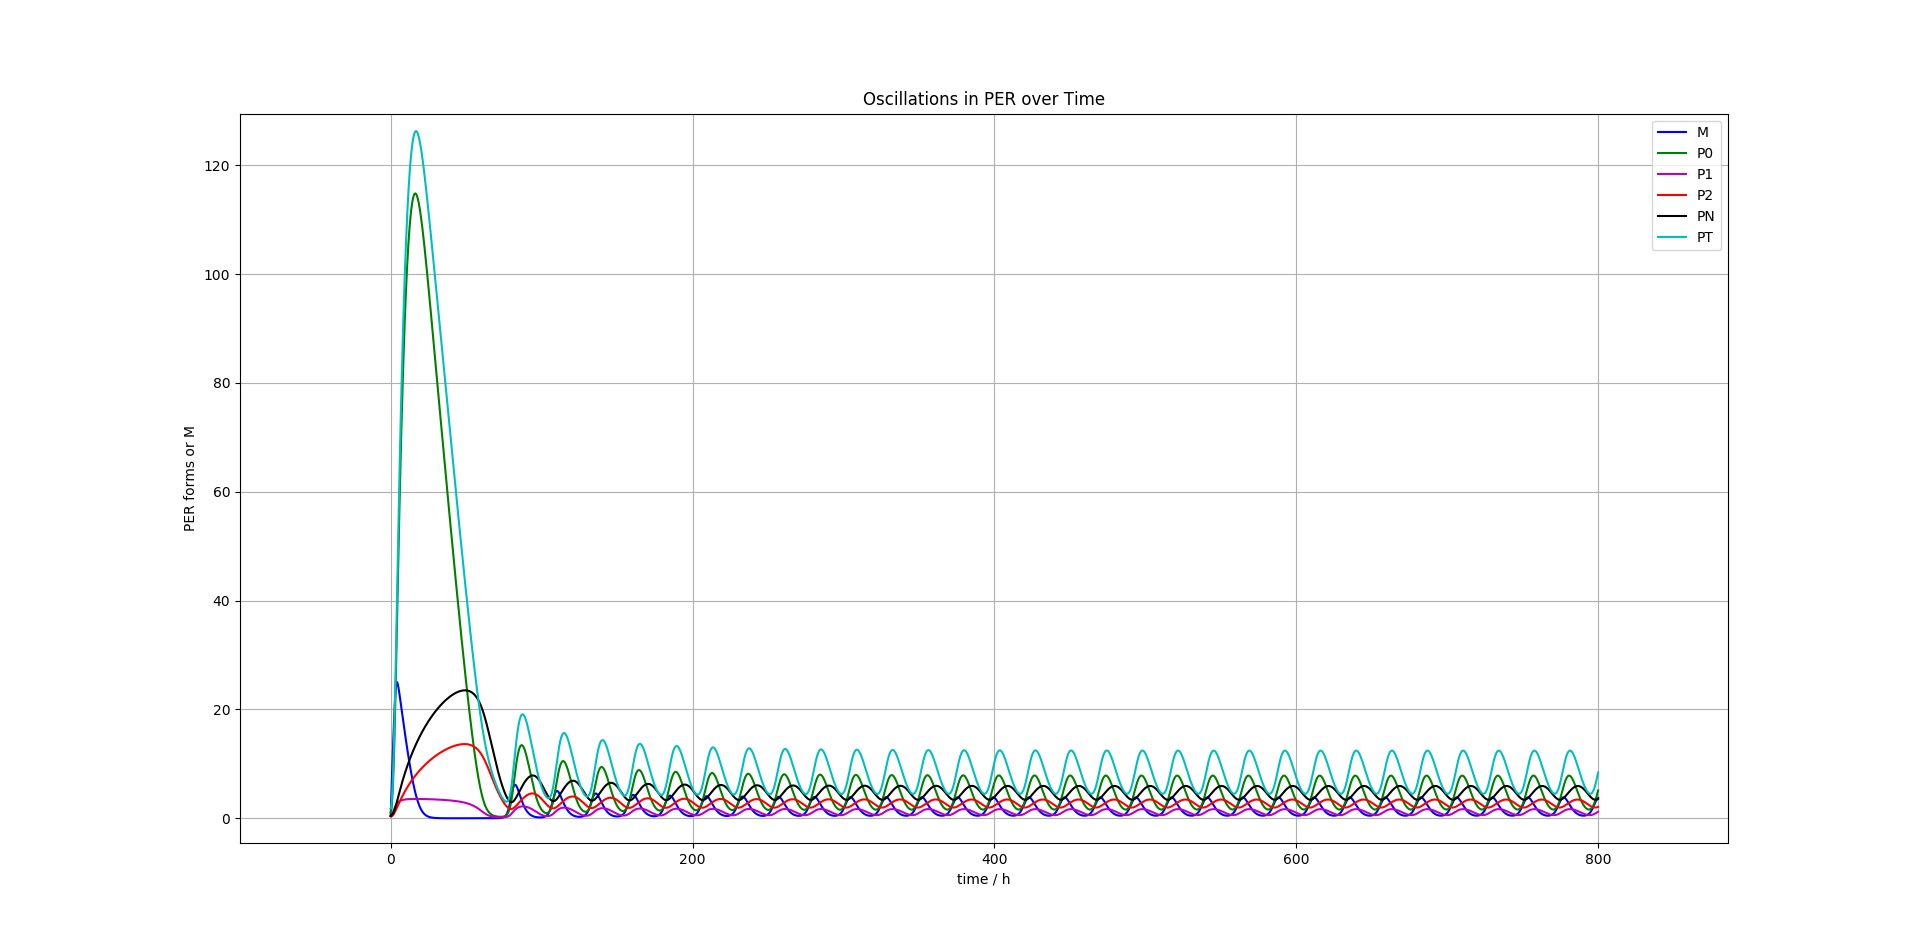
\includegraphics[width=\linewidth]{{"../plots/es_1.1"}.png}
	\caption{A simulation of the Goldbeter fly model using parameters (found using an evolutionary strategy): $n$ : $9.71$, $K_1$ : $10.00$, $K_2$ : $10.00$, $K_3$ : $8.31$, $K_4$ : $9.38$, $K_m$ : $9.06$, $K_d$ : $2.16$, $K_I$ : $1.52$, $V_1$ : $8.26$, $V_2$ : $2.17$, $V_3$ : $4.36$, $V_4$ : $7.82$, $v_m$ : $5.51$, $v_d$ : $5.70$, $v_s$ : $7.34$, $k_1$ : $7.77$, $k_2$ : $1.29$, $k_s$ : $1.11$}
	\label{fig:es1.1}
\end{figure}

\section{Discussion}

\end{document}